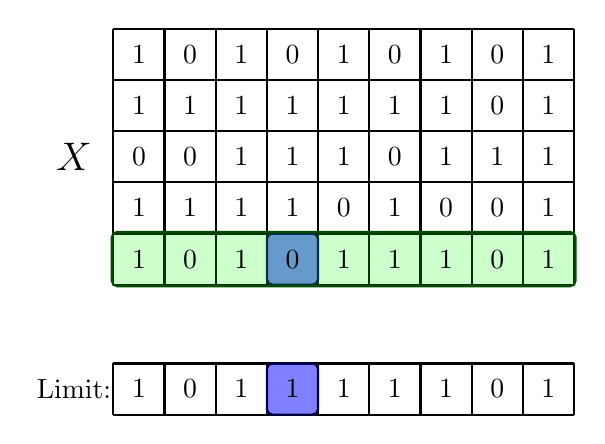
\begin{tikzpicture}
    \def\elements{{
            {1, 1, 0, 1, 1},
            {0, 1, 0, 1, 0},
            {1, 1, 1, 1, 1},
            {0, 1, 1, 1, 0},
            {1, 1, 1, 0, 1},
            {0, 1, 0, 1, 1},
            {1, 1, 1, 0, 1},
            {0, 0, 1, 0, 0},
            {1, 1, 1, 1, 1}
        }}
    \def\result{{1, 0, 1, 1, 1, 1, 1, 0, 1}} 
    \def\n{8}
    \def\m{4}
    \def\step{0.65}

    \draw[step = \step, thick] (0, 0) grid ({\step * (\n + 1)}, {-\step * (\m + 1)});
    \draw[thick, blue!30!black, rounded corners = 2pt, fill = blue, fill opacity = 0.5]
        (3 * \step, {-\step * (\m + 1)}) rectangle (4 * \step, {-\step * \m});
    \draw[thick, green!30!black, rounded corners = 2pt, fill = green, fill opacity = 0.2]
        (-0.02, {-\step * (\m + 1) - 0.02}) rectangle ({\step * (\n + 1) + 0.02}, {-\step * \m + 0.02});
    
        
    \foreach \i in {0, 1, ..., \n}{
        \foreach \j in {0, 1, ..., \m}{
            \node at ({\step / 2 + \i * \step}, {-\step / 2 - \j * \step})
                {\pgfmathparse{\elements[\i][\j]}\pgfmathresult};
        }
    }

    \begin{scope}[shift = {(0, {-\step * (\m + 1) - 1})}]
        \draw[step = \step, thick] (0, 0) grid ({\step * (\n + 1)}, -\step);
        \draw[thick, blue!30!black, rounded corners = 2pt, fill = blue, fill opacity = 0.5]
            (3 * \step, 0) rectangle (4 * \step, -\step);
            
        \foreach \i in {0, 1, ..., \n}{
            \node at ({\step / 2 + \i * \step}, {-\step / 2})
                {\pgfmathparse{\result[\i]}\pgfmathresult};
        }
    \end{scope}

    \node at (-0.5, {-\step * (\m + 1) / 2}) {\Large $X$};
    \node at (-0.5, {-\step * (\m + 1.5) - 1}) {Limit:};

\end{tikzpicture}